\section{Challenges of Eigenvalue Based MOE}
\label{sec:challenges_moe}

\subsection{Degradation of the Eigenstructure through Sub-Sampling}

The application of classical \glspl{ic} such as \gls{aic} and \gls{mdl} for model order estimation critically depends on the
soundness of the re-parameterization of the maximum likelihood function introduced in~\autoref{eq:max_likelihood}.
While robust and effective for coherently sampled covariance matrices, this methodology loses its validity
due to the severely increased challenge in capturing the true eigenstructure of the covariance matrix \( \bfm{C}_x \)
when sub-array sampling is employed~\cite{barthelme21sub}.

Barthelme et al.~\cite{barthelme21sub} asserted that the eigenstructure of the sub-sampled covariance matrix \( \Csub \)
can no longer be decomposed into signal and noise subspaces when the model order \( N \) exceeds the number of RF
chains \( L \).\\
In contrast, Meyer~\cite{meyer} demonstrated the convergence of \( \Csub \rightarrow \bfm{C}_x \) as \( K \rightarrow \infty \).
It is thus obvious that the sub-sampled covariance matrix's eigenstructure must still posses the capacity to encode
the coveted information (\( \{ \bfT_n :\, n \in \{1, \ldots, N\} \} \)). \\
This convergence, however, unfolds asymptotically and at a pace that challenges its practical utility in real-world scenarios.

The progression from theoretical considerations to empirical observations underscores the practical dilemmas posed by
sub-array sampling. The fidelity with which \( \Csub \) mirrors \( \bfm{C}_x \) is notably compromised, as it not only
loses positive semi-definiteness but also introduces a broader dispersion of the noise eigenvalues \( \bfL_{\eta} \).
This dispersion deviates from their expected individual normal distributions around the noise variance \( \sigma^2_\eta \)~\cite[Chapter 6]{meyer}.

These revelations prompt critical inquiry into the manifestation and progression of information loss within the
eigenstructure of \( \Csub \), especially under finite snapshot conditions. \\
Does this information loss occur abruptly with the emergence of negative eigenvalues, or does it manifest more gradually,
with eigenvalues slowly diverging from those of \( \bfm{C}_x \)?


\subsubsection{Distribution of the noise eigenvalues}
\label{subsub:noise_eigval_distrib}
\begin{figure}[H]
    \centering
    \subfloat[]{{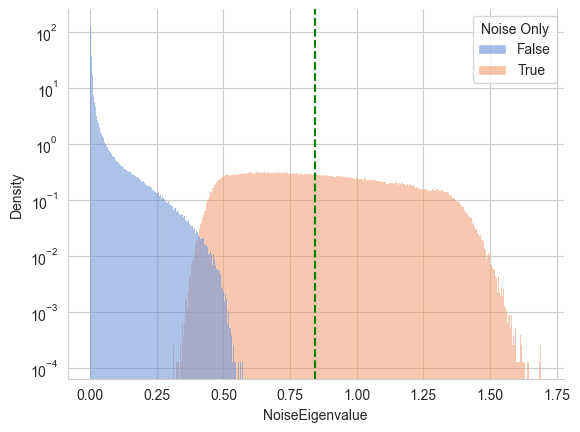
\includegraphics[width=0.5\textwidth]{figures/04_ModelOrderEstimation/noise_eigval_distrib.png}}}
    % \hspace{0.5cm}
    \subfloat[]{{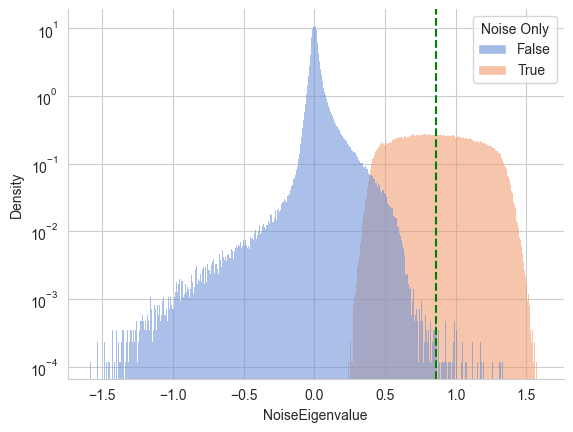
\includegraphics[width=0.5\textwidth]{figures/04_ModelOrderEstimation/noise_eigval_distrib_sub.png}}}
    \caption{Density estimates of noise eigenvalues of the full (a) and sub-sampled (b) covariance matrices, and \( K = 100 \).}
    \label{fig:noise_eigval_distrib}
\end{figure}

\autoref{fig:noise_eigval_distrib} depicts the density estimates of noise eigenvalues for both full and sub-sampled
covariance matrices, given a set number of snapshots \( K = 100 \).
The dataset was generated with a specified noise level of \( P_\eta = -120 \, \si{\deci\bel}_{(\si{\micro\volt})} \),
equating to a noise variance of \( \sigma^2_\eta = 1 \si{\micro\volt\squared} \). \\
The theoretical expectation for the distribution of the noise eigenvalues is given by~\autoref{eq:eigval_superimposed} and
assumes normally distributed noise eigenvalues around \( \sigma^2_\eta \).\\
In the noise-only case, where no signals are present (\( N = 0 \)), the orange distributions indeed aligns with this prediction.
However, the blue distribution, representing scenarios with one to five signals (\( N \in \{1, \ldots, 5\} \)), deviates
from this pattern.

\begin{figure}[H]
    \centering
    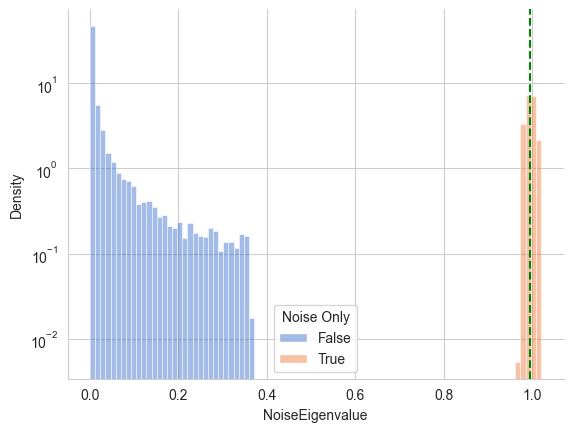
\includegraphics[width=0.45\textwidth]{figures/04_ModelOrderEstimation/noise_eigval_distrib_100k.png}
    \caption{Distribution of noise eigenvalues for \( K = 1e5 \).}
    \label{fig:noise_eigval_distrib_100k}
\end{figure}
Notably, with an increased snapshot count (\( K = 1e5 \)), depicted in \autoref{fig:noise_eigval_distrib_100k}, the
central tendency of the noise eigenvalues for \( N = 0 \) shifts closer to \( \sigma^2_\eta \) which is
in line with expectations. However, the separation between the two clusters—one corresponding to the noise-only case and
the other where signals are present— cannot be explained by the theoretical expectations. \\
Considering that this behavior is consistent across independent simulation environments, it is reasonable to assume that
this bifurcation cannot be explained by a simple ``bug'' in either simulation environment.\\

\subsubsection{Influence of the Model Order}
The emergence of negative eigenvalues within sub-sampled covariance matrices exhibits a strong correlation with the
true model order \( N \). As the complexity of the underlying model increases, the fidelity of the estimated sub-sampled covariance matrix
\( \Csub \) to the true covariance matrix \( \bfm{C}_x \) deteriorates \(\sim\: N \uparrow\; \rightarrow \; \mathcal{L}(\bfm{C}_x, \Csub) \uparrow \).\\
This deterioration is manifested through an increased likelihood of \( \Csub \) losing its positive semi-definiteness.

\begin{figure}[H]
    \centering
    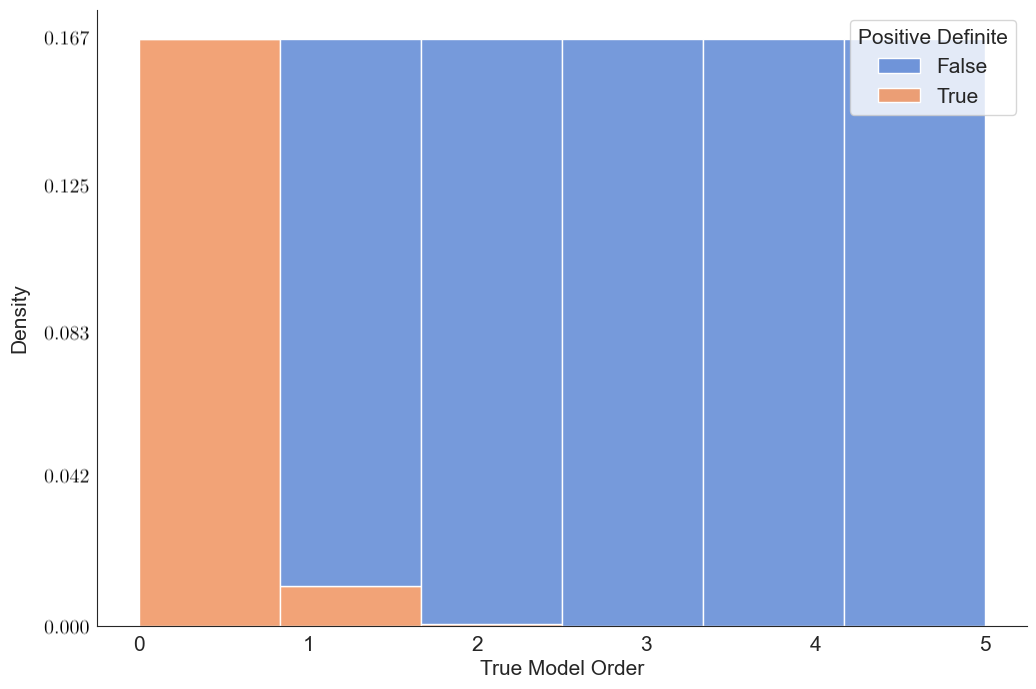
\includegraphics[width=0.45\textwidth]{figures/04_ModelOrderEstimation/eigval_PD_N.png}
    \caption{Illustration of the declining positive definiteness with increasing model order \( N \).}
    \label{fig:eigval_pd_n}
\end{figure}

\autoref{fig:eigval_pd_n}%
\footnote{The data depicted in \autoref{fig:eigval_pd_n} originates from the dataset \( \DMain_{(\text{test})} \), which is discussed in~\autoref{ch:dataset_generation}.}
demonstrates that, at \( K = 100 \), a considerable majority of samples with \( N > 0 \)
experience a loss of positive semi-definiteness in the sub-sampled covariance matrix. \\
Nonetheless, as detailed in~\autoref{ch:evaluation_results}, obtaining reliable model order estimates remains feasible
using the \gls{aic} and \gls{mdl} criteria for most samples where the model order \( N \) is less than the number of RF chains (\( N < L = 3 \)). Furthermore, both the \gls{eft} and deep learning models have been shown to provide accurate model order estimates for \( N \leq 3 \). Empirical evidence indicates that
the eigenvalues retain the ability to encapsulate essential information, enabling accurate predictions of \( N \) even when \( N > 3 \).


\begin{figure}[H]
    \centering
    \subfloat[]{{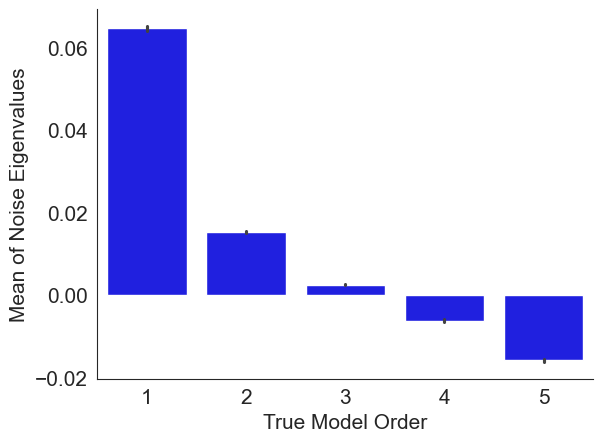
\includegraphics[width=0.37\textwidth]{
        figures/04_ModelOrderEstimation/noise_mean_N.png
    }}}
    \subfloat[]{{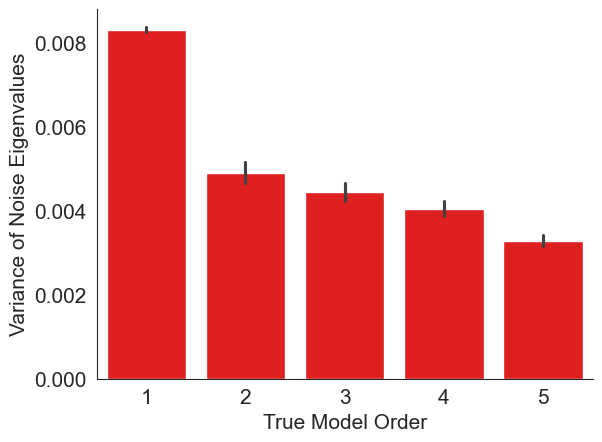
\includegraphics[width=0.37\textwidth]{
        figures/04_ModelOrderEstimation/noise_var_N.png
        }}}
    \caption{
        Mean (a) and variance (b) of the noise eigenvalues for varying model orders \( N \).
    }
    \label{fig:noise_eigval_mean_var_vs_N}
\end{figure}

\autoref{fig:noise_eigval_mean_var_vs_N} illustrates the mean and variance of the noise eigenvalues for varying model orders \( N \).
For sake of interpretability of the linearly scaled y-axis, the mean of the noise eigenvalues for \( N = 0 \) has been omitted from
the plot. \\
The clear correlation between the model order \( N \) and the mean and variance of the noise eigenvalues, can be interpreted
as evidence that the sought-after information about the model order is still encoded within the eigenstructure of the sub-sampled
covariance matrix. Another positive observation is that the \( 95\% \) confidence intervals of mean, as well as the variances
are approximately an order of magnitude smaller than the mean values.

\subsubsection{Influence of the SNR and Number of Snapshots}
% However, to fully comprehend the implications of these findings, it is essential to first
% understand the statistical distributions of minimum and maximum \glspl{snr}, along with the \gls{sir}, and how they
% correlate with the model order \( N \). This is discussed in~\autoref{subsub:snr_sir_distrib}.
Considering that positive definiteness of the covariance matrix seems only to occur for \( N \leq 1 \) for \( K = 100 \),
an evaluation of the relationship between the \gls{sir} and the probability of encountering negative eigenvalues
does not seem to be particularly insightful.\\
However, since both the \( \SNRmin \) and \( \SNRmax \) can already be defined for \( N = 1 \), it appears worthwhile to
investigate the influence of the \gls{snr} on the occurrence of negative eigenvalues.

\begin{figure}[H]
    \centering
    \subfloat[]{{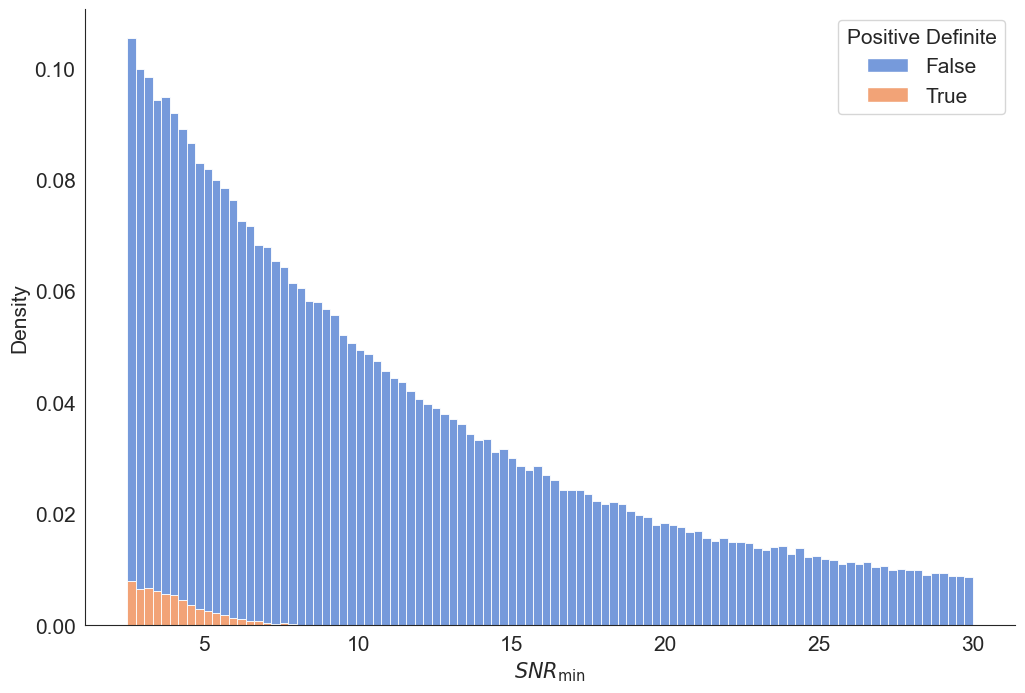
\includegraphics[width=0.33\textwidth]{figures/04_ModelOrderEstimation/snr_hist/min_PD.png}}}
    % \hspace{0.5cm}
    \subfloat[]{{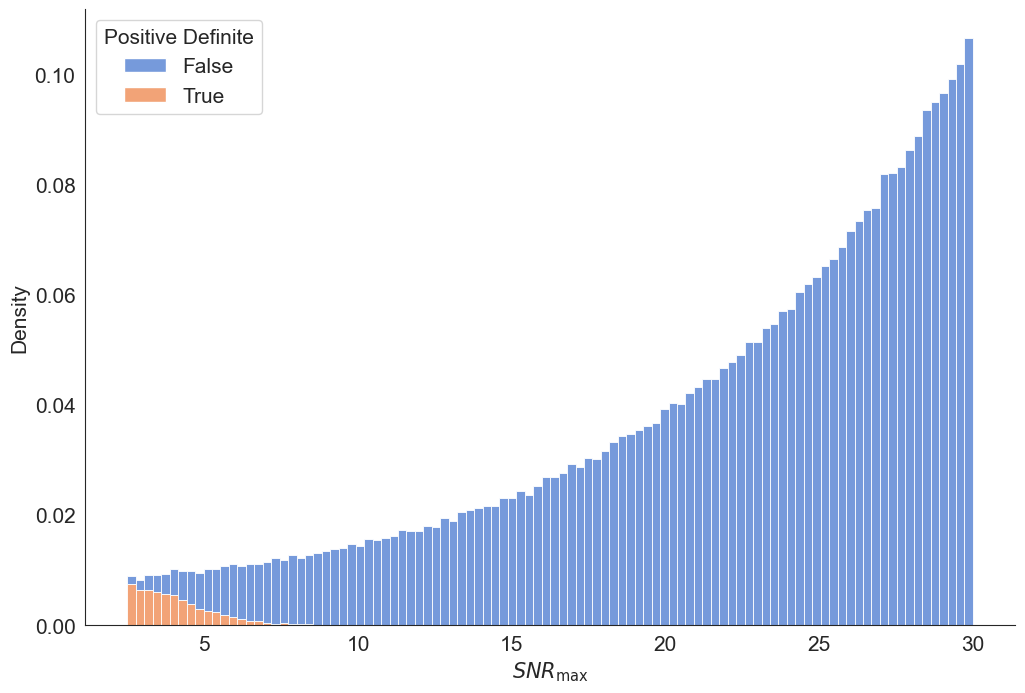
\includegraphics[width=0.33\textwidth]{figures/04_ModelOrderEstimation/snr_hist/max_PD.png}}}
    \caption{Histograms of the \( \SNRmin \) (a), \( \SNRmax \) (b), differentiated w.r.t.\ the positive definiteness.}
    \label{fig:snr_sir_hist}
\end{figure}

\autoref{fig:snr_sir_hist} illustrates the histograms of the \( \SNRmin \) and \( \SNRmax \) values, differentiated with
respect to the positive definiteness of the sub-sampled covariance matrix. \\
As elucidated in the previous chapter, the \gls{pdf} of the \gls{snr} is expected to be a uniform distribution. Utilizing
this knowledge to interpret the histograms, it is evident, that \( \Csub \) quickly loses its positive semi-definiteness
for increasing \( \SNRmin \) and \( \SNRmax \) values.\\


Further insights into the occurrence of negative eigenvalues can be gained by investigating the influence of the number of
snapshots \( K \). Our theoretical expectation is that the sub-sampled covariance matrix should converge asymptotically to the true covariance
matrix -- \( \Csub \rightarrow \bfm{C}_x \) as \( K \rightarrow \infty \). \\
We will therefore investigate the probability of encountering negative eigenvalues for varying numbers of snapshots \( K \)
on the dataset \( \DKvar \) for \( 1 \leq K \leq 1000 \). Subsequently, we will include the \gls{snr} into this evaluation
and present a two-dimensional analysis of the occurrence of negative eigenvalues.

\begin{figure}[H]
    \centering
    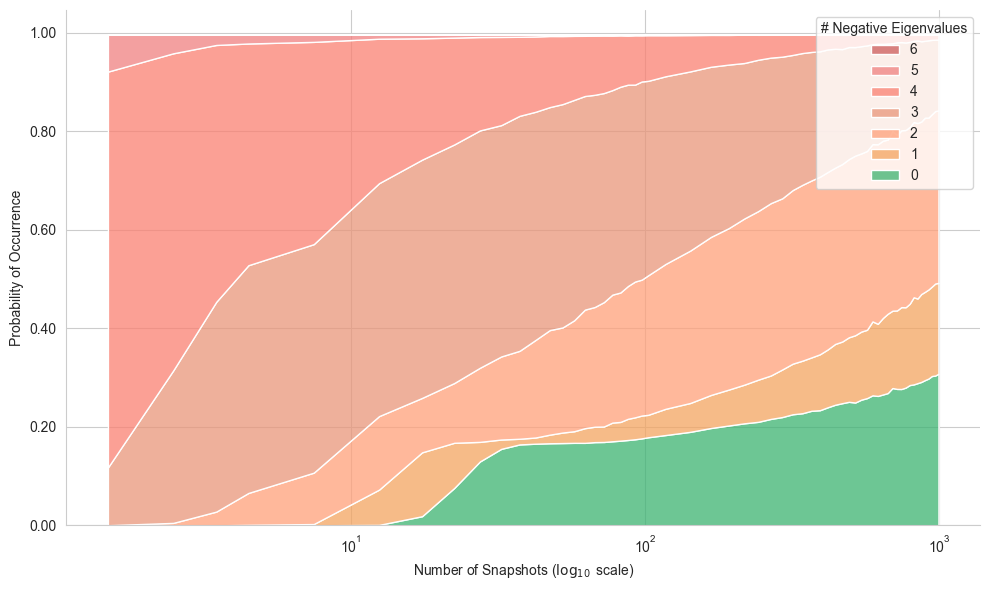
\includegraphics[width=0.8\textwidth]{figures/04_ModelOrderEstimation/num_neg_eigvals_vs_K.png}
    \caption{Probability of encountering \( \ell_{\textit{neg}} \) negative eigenvalues for varying numbers of snapshots \( K \).}
    \label{fig:num_neg_eigvals_vs_K}
\end{figure}

\autoref{fig:num_neg_eigvals_vs_K} illustrates that the likelihood of \( \Csub \) being positive semi-definite asymptotically
increases with \( K \), aligning with theoretical insights presented in~\cite{meyer}.
According to the observations, depicted in~\autoref{fig:eigval_pd_n}, the probability of encountering negative eigenvalues
at \( K = 100 \) should be approximately
\[
    \Pr(\ell_{\textit{neg}} > 0|K=100) = 1 - \Pr(\ell_{\textit{neg}} = 0| K=100) \approx  1 - (0.1\overline{6} + 0.01) = 0.82\overline{3}.
\]

Given the close agreement between both%
\footnote{\autoref{fig:eigval_pd_n} being observed on \( \DMain_{(\text{test})} \) and \autoref{fig:num_neg_eigvals_vs_K} on \( \DKvar \) for \(K = 100\).}
observed probabilities, we are poised to continue with the two-dimensional analysis.



\begin{figure}[H]
    \centering
    \subfloat[]{{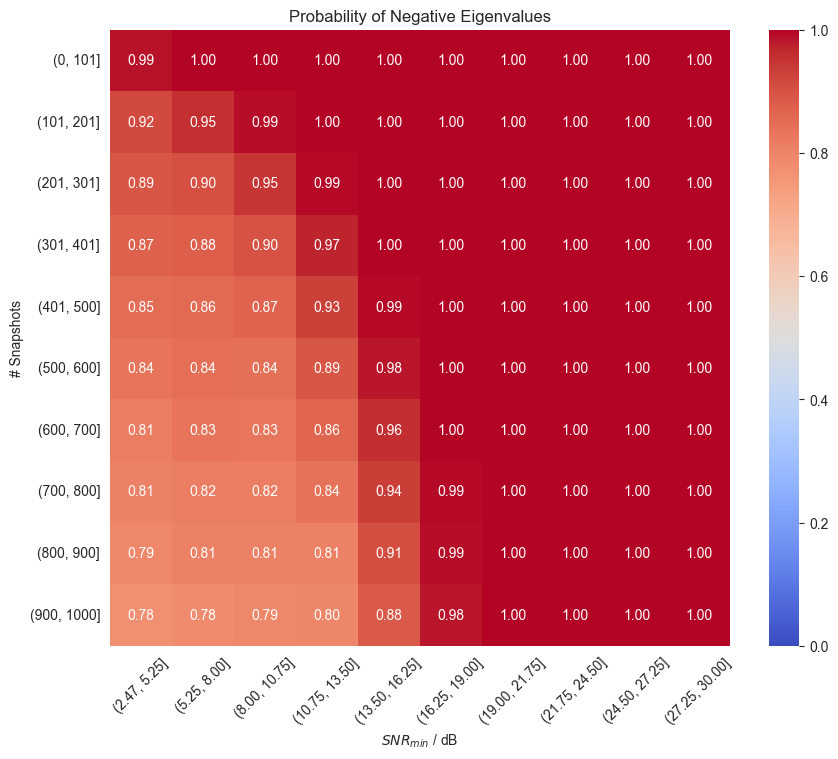
\includegraphics[width=0.45\textwidth]{figures/04_ModelOrderEstimation/snr_min.png}}}
    % \hspace{0.5cm}
    \subfloat[]{{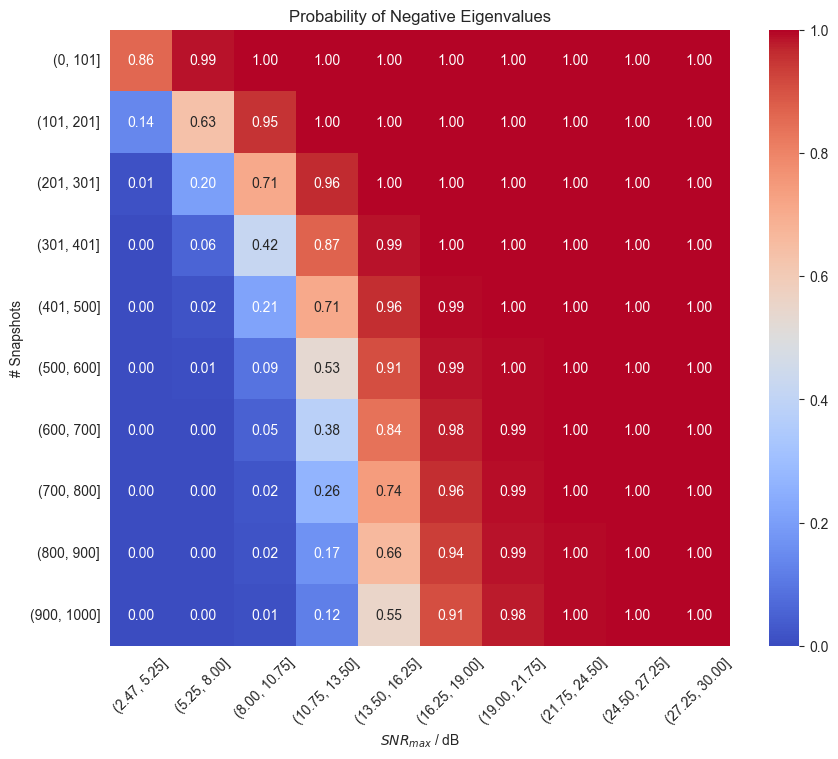
\includegraphics[width=0.45\textwidth]{figures/04_ModelOrderEstimation/snr_max.png}}}
    \caption{Probabilities of negative eigenvalues for the minimum (a) and maximum (b) \gls{snr}, for a varying number
    of snapshots.}
    \label{fig:snr_num_snapshots_pd}
\end{figure}

\autoref{fig:snr_num_snapshots_pd} shows that high \( \SNRmin \) and \( \SNRmax \) values strongly correlated with a
higher probability of negative eigenvalues. Whereas the \( \Pr(\ell_{\textit{neg}} > 0) \) seems to be mostly dependent
on \( N \) for \( K = 100 \), it is evident that other even hg


\subsubsection{Handling Negative Eigenvalues}
To still be able to use the beforementioned algorithmic methods, the eigenvalues need to be transformed so that the resulting
vector \( \bfL \) only contains non-negative values.
Since the \gls{aic}, \gls{mdl}, and \gls{eft} cannot cope with non-positive eigenvalues, they had to be inferred from transformed
eigenvalues \( \widetilde{\bfL} \) whose positivity was ensured according to~\autoref{eq:pos_eigvals}.

\begin{align}
    \widetilde{\bfm{\lambda}} &=
    \begin{cases}
      \bfm{\lambda} + \lambda_M + \epsilon_{\text{eft}} & \text{if } \lambda_M \leq \epsilon_{\text{eft}} \text{ for \gls{eft}}, \quad \epsilon_{\text{eft}} = \num{1e-6} \\
      \bfm{\lambda} + \lambda_M + \epsilon_{\text{IC}} & \text{if } \lambda_M \leq \epsilon_{\text{IC}} \text{ for \gls{aic} and \gls{mdl}}, \quad \epsilon_{\text{IC}} = \num{1} \\
      \bfm{\lambda} & \text{otherwise}
    \end{cases}
    \label{eq:pos_eigvals}
\end{align}

The additional offset term \( \epsilon_{\text{IC}} \) was introduced to ensure that \( \widetilde{\bfm{\lambda}}_{\text{IC}} \)
does not contain any values close to zero, which would result in most criteria values \( \bfm{\mathrm{AIC}}[n] \)  and \( \bfm{\mathrm{MDL}}[n] \) diverging to
\( \infty \). Lower values of \( \epsilon_{\text{IC}} \) appear to be correlated with a higher bias. A value of \( \epsilon_{\text{IC}} = 1 \) was chosen,
since \( \sigma^2_{\eta} = 1 \), and therefore the noise eigenvalues \( \bfm{\lambda}_{\eta} \) are expected to cluster around 1.\\
\gls{mdl} exhibited a slightly better performance in terms of bias and variance for eigenvalues \( \widetilde{\bfL} \) being
transformed by
\begin{equation}
    \mathcal{TF} \coloneq \{\| \bullet \| \rightarrow \text{sort}(\bullet) \rightarrow \bullet = \bullet + \epsilon_{\text{IC}}\}, \quad \mathcal{TF} : \bfL \mapsto \widetilde{\bfL}.
\end{equation}
The \gls{eft}, conversely, only requires a small offset to ensure that the eigenvalues are greater than zero. Increasing
the offset reduces the goodness of fit of the \gls{eft}'s predicted eigenvalue profile to the true eigenvalues.

% \section{Factors Influencing \gls{moe}}
% The \gls{moe} methods discussed in this thesis depend on the distribution of eigenvalues. Important factors influencing \gls{moe}
% include the \glsfirst{snr}, \glsfirst{sir}, the array's aperture \( D \), finite-sample effects when \( K < 10M \),
% modeling errors, and the impact of sub-sampling. As the conventional methods used at Rohde \& Schwarz are affected by
% these factors, they will be discussed further at the end of this chapter~\cite{meyer}.\\


% - multipath -> rank deficient -> overfitting -> higher model order: `By partitioning the whole array into sub-
% arrays and averaging of the sub-array received covariance matrices, the equivalent source covariance matrix becomes
% nonsingular. The FBSS scheme is widely-used since it can be regarded as a preprocessing before applying AIC and MDL [9]
% as well as DOA estimation algorithms`'\cite{yang2020}